\chapter{Нелинейные колебания оболочек}\label{ch:ch3}

\section{Обзор} \label{ch:ch3/sec1}

{\color{blue}
В данной вводной части будет уделен акцент в основном пластинам и оболчкам из ФГМ, и немного затронуты оболочки из композиционного материала, но можно распространить и на други виды конструкций и материалов.


Произведем беглый обзор литературы посвященой геометрически нелинейным свободным и вынужденным колебаниям оболочек из традиционных и современных материалов. Плоские и несовершенные пластины и мембраны исключены из рассмотрения. В общем виде рассматриваются замкнутые оболочки и изогнутые панели из функционально-градиентных и композитным материалов; внимание уделяется нелинейным колебаниям оболочек. Теоретические, численные и экспериментальные исследования посвященные конкретным динамическим проблемам, включающим параметрические колебаний, устойчивости, динамического смятия, нестационарных колебаний и хаотические колебания.
}

Оболочечные конструкции используются в самолетах, космических аппаратах, ракетах, автомобилях, компьютерах, подводных лодках, катерах, резервуарах для хранения и даже крышах зданий.

В последнее десятилетие непрерывное развитие материаловедения и инженерии, наряду с растущим спросом на производство легких конструкций, привело к использованию передовых материалов (слоистых композитов и функционально-градиентных материалов (ФГМ)) при проектировании оболочечных конструкций. Среди разнообразных областей применения, аэрокосмическая и авиационная области являются особенно сложными, так как они включают в себя взаимодействие жидкостей  и конструкции и использование новых материалов с мало-известными свойствами. Для этого необходимо разрабатывать модели, учитывающие нелинейные эффекты, такие как большие деформации, а также уметь предсказывать реакцию конструкции на большие амплитудные колебания.


В случае линейных колебаний замкнутых (по окружности) цилиндрических оболочек, подверженных радиальным периодическим возбуждениям, форма моды оболочки представляет собой стоячую волну, непосредственно возбуждаемую внешним возбуждением, которая представляет собой число \(n\) узловых диаметров. Такая мода называется вынужденной. При колебаниях оболочек с большой амплитудой существует внутренний резонанс один к одному между \textbf{управляемой} модой и ортогональной модой, имеющей ту же форму и собственную частоту, что и управляемая мода, но повернутой на \(\pi/2n\), известной как \textbf{сопутствующая} мода. 

Такое взаимодействие мод приводит к появлению отклика бегущей волны в окружном направлении оболочки, который проявляется даже при амплитудах колебаний, меньших, чем толщина оболочки. Фактически, наличие отклика бегущей волны вблизи резонанса имеет принципиальное отличие от линейных колебаний. 


Другой важной особенностью замкнутых круговых цилиндрических оболочек при колебаниях большой амплитуды является динамическое осесимметричное сжатие, которое было рассмотрено как теоретически, так и экспериментально. В частности, при колебаниях большой амплитуды оболочка испытывает внутреннее осесимметричное динамическое сжатие с удвоенной частотой возбуждения, что гарантирует квазинерастяжимость оболочки в плоскости. Без этого осесимметричного сжатия оболочка значительно увеличила бы свою длину по окружности, что противоречит механике оболочек. На самом деле, оболочки легче изгибаются, чем растягиваются.

Оболочки подверженные нагрузкам в плоскости, теряют устойчивость и разрушаются после определенного порога. Фактически, при наличии статических нагрузок в плоскости неустойчивость возникает через вилообразную бифуркацию (Pitchfork bifurcation), в то время как при периодических нагрузках в плоскости так называемая параметрическая неустойчивость возникает через бифуркацию удвоения периода в соседней области частот, вдвое превышающей собственные частоты изгибной моды. В последнем случае, в отличие от нелинейных колебаний оболочек из-за радиального гармонического возбуждения, неустойчивость может возникнуть даже при малых амплитудах возбуждения и намного ниже статической нагрузки смятия.


Оболочки, заполненные жидкостью, имеют более низкие собственные частоты вследствие дополнительной виртуальной массы самой жидкости. В цилиндрических оболочках эффект добавленной виртуальной массы ниже для асимметричных мод, чем для осесимметричных мод. Поэтому нелинейность, проявляемая тонкими замкнутыми круговыми оболочками, усиливается присутствием вязкой жидкости. Более того, круговые цилиндрические оболочки, поддерживаемые или зажатые с обоих концов и транспортирующие жидкость, теряют устойчивость через дивергенцию, которая представляет собой статическую вилообразную бифуркацию равновесия, когда скорость потока  достигает критического значения. Дивергенция является сильно субкритической, становясь сверхкритической для высоких скоростей потока flow.  В этом случае система имеет два или более устойчивых решений, связанных с дивергенцией, намного раньше, чем возникает вилочная бифуркация. Другими словами, если оболочка возмущена от начальной конфигурации, она может иметь сильные деформации, приводящие к разрушению намного ниже критической скорости, которая может быть предсказана линейным анализом.

В отличие от замкнутых круговых цилиндрических оболочек, криволинейные панели (т.е. открытые оболочки, с одинарной и двойной кривизной) не всегда демонстрируют внутренний резонанс, если только для определенных соотношений толщины и площади, и не имеют осесимметричного динамического сжатия.  Особенности панелей, которые делают нелинейный анализ этих структур интересным, - это асимметричный характер колебаний относительно исходной недеформированной средней поверхности, нелинейное поведение смягчения, переходящее в упрочнение при колебаниях большой амплитуды, и различные условия внутреннего резонанса, которые могут иметь место для различных форм.


\subsection{Краткий обзор нелинейных теории оболочек} \label{ch:ch3/sec1/sub1}

Классические теории нелинейной механики оболочек, подходящие для тонких оболочек, включают теории Доннелла \cite{donnel1934}, Новожилова \cite{novozhilov1953}, Сандерса \cite{sanders1963}, Койтера \cite{koiter1966} и Флюгге Лурье Бирна \cite{ginsberg1973}, которые все основаны на гипотезах Кирхгофа-Лява. В частности, нелинейная теория мелких оболочек Доннелла пренебрегает инерцией в плоскости и дает точные результаты только для очень тонких оболочек. В этой теории смещения в плоскости являются бесконечно малыми, в то время как поперечные смещения порядка толщины оболочки. Более того, нелинейные члены сохраняются только в поперечном сдвиге (нелинейные члены типа фон Кармана, по аналогии с рассмотрением пластин); однако другие эффекты, такие как нелинейность, связанная с плоскими смещениями, игнорируются. Теория Доннелла, без гипотезы тонкой оболочки, сохраняет инерцию в плоскости и является более точной, чем нелинейная теория тонкой оболочки Доннелла; однако, она сохраняет нелинейные члены только типа фон Кармана. Теория Сандерса - это более расширенная нелинейная теория оболочек, разработанная Сандерсом \cite{sanders1963} первоначально в тензорной форме. Эта же теория была получена независимо Койтером \cite{koiter1966} примерно в тот же период, что привело к обозначению этой теории как нелинейной теории оболочек Сандерса-Койтера. Эта теория подходит для конечных перемещений с малыми деформациями и умеренно малыми вращениями. Поэтому в теории Сандерса-Койтера смещения в плоскости не являются бесконечно малыми, а в соотношениях деформационных смещений существуют нелинейные члены, которые зависят как от смещений в плоскости, так и от поперечных смещений. В теориях Доннелла и Сандерса-Койтера изменения кривизны и кручения средней поверхности предполагаются линейными. Более того, теория Сандерса-Койтера дает точные результаты для амплитуд колебаний, значительно превышающих толщину оболочки, в то время как теория Доннелла точна только для очень тонких оболочек и мод с высоким окружным числом волн.


Общие нелинейные теории оболочек, разработанные Новожиловым \cite{novozhilov1953}, и теория Флюгге-Лур'е-Бирна \cite{ginsberg1973} очень похожи и отличаются только в плане замены кривизны и кручения. В обеих теориях можно сохранить нелинейность в изменениях кривизны и кручения \cite{amabili2008}. Более того, предположение о тонкости сохраняется в выводах обеих теорий, а соотношения деформационных сдвигов включают нелинейности как в поперечных, так и в плоских перемещениях. Все эти классические теории получены путем пренебрежения деформацией поперечного сдвига и инерцией вращения, и поэтому могут давать неточные результаты для умеренно толстых или слоистых анизотропных оболочек. Для того чтобы преодолеть это ограничение, были введены теории сдвиговой деформации. Эти теории можно разделить на теории деформации сдвига первого порядка и теории деформации сдвига более высокого порядка; в первой категории для равновесия требуется поправочный коэффициент сдвига, поскольку предполагается равномерная деформация сдвига по толщине оболочки. Теории деформации сдвига более высокого порядка преодолевают это ограничение, поскольку предполагается реалистичное распределение напряжения сдвига по толщине оболочки, что также удовлетворяет условию нулевого напряжения сдвига на верхней и нижней поверхностях оболочки. Эти теории были полностью рассмотрены в книгах Амабили \cite{amabili2008}, Редди \cite{reddy2004} и Каррера и др \cite{carreranali2011}. Более того, теории линейной сдвиговой деформации и зигзагообразной деформации (слои с постоянным углом сдвига) были подробно рассмотрены Каррерой \cite{carrera2002, carrera2003},  и Редди и Арсиньегой \cite{reddyarciniega2004}.


Нелинейная теория деформации сдвига первого порядка была впервые предложена Редди и Чандрашекхарой [18] и основана на нелинейных членах Сандерса-Койтера. Для описания деформаций оболочки использовались пять независимых переменных: три перемещения и два вращения. Нелинейная теория сдвиговых деформаций оболочек первого порядка, основанная на нелинейных членах типа фон Кармана, и ее формулировки в виде отдельных элементов также приведены в работе Редди [13]. Либреску [19] разработал нелинейную теорию оболочек, расширив смещения оболочки кубическими членами в поперечной координате. Деннис и Палазотто [20] и Палазотто и Деннис [21] расширили линейную теорию оболочек Редди высшего порядка со сдвиговой деформацией до нелинейной деформации, введя нелинейные члены типа фон Кармана. Нелинейная теория оболочек высшего порядка для многослойных анизотропных оболочек с поперечно сжимаемым ядром была разработана Хохе и Либреску [22]. В их теории гипотезы Кирхгофа-Лява были приняты для торцевых поверхностей, а для перемещений ядра рассматривалось разложение в ряд мощности второго/третьего порядка. Чаудхури [23] разработал теорию нелинейного зигзага для нелинейного конечно-элементного анализа двояковыпуклых оболочек путем рассмотрения полных нелинейных соотношений деформационных перемещений для пяти независимых переменных оболочки. Амабили и Редди [24] разработали новую теорию для закрытых и открытых оболочек, которая, в отличие от предыдущих нелинейных теорий оболочек, была выведена с сохранением инерции вращения, деформации сдвига и нелинейности в плоскости и поперечных смещениях. Новая теория показала превосходство над существующими нелинейными теориями деформации сдвига при прогнозировании колебаний большой амплитуды глубоких и умеренно толстых ламинированных круговых цилиндрических оболочек [25] и изогнутых панелей [26]. Недавно Амабили [27] расширил теорию [24], добавив эффект растяжения толщины и приняв во внимание геометрические несовершенства. В этой новой теории для описания деформации оболочки использовались шесть независимых переменных. В частности, в [27] предполагается равномерная поперечная нормальная деформация по всей толщине оболочки. Эта теория была расширена до поперечной нормальной деформации третьего порядка Амабили [28]. Преимущества теорий оболочек, сохраняющих поперечные нормальные напряжения и деформации, заключаются в использовании полных трехмерных определяющих уравнений, и они особенно подходят для мягких материалов, таких как резины и биологические материалы, где достигаются очень большие деформации, сопровождающиеся большим уменьшением толщины. Parisch [29] и Sansour [30] разработали независимые теории оболочек, которые вводят квадратичное предположение о смещении оболочки по толщине оболочки. Более того, точная линейная теория оболочек, учитывающая изменение толщины, была разработана Каррерой и другими [31] и Феррейрой и другими [32]. Геометрически нелинейные теории оболочек на тензорной основе достаточно широко представлены в литературе [33 45]. Еремеев и Петрашкевич [33] разработали общую нелинейную теорию оболочек с учетом фазовых переходов материалов. В их теории смещения оболочек выражались через усредненные по работе переводы и повороты поперечных сечений оболочек. Более того, все связи оболочек были найдены из вариационного принципа стационарной потенциальной энергии. Опока и Петрашкевич [34] последовательно получили полную краевую задачу для нелинейной теории тонких упругих оболочек, выраженную в терминах результирующих напряжений и изгиба опорной поверхности оболочки. Арсиньега и Редди [35] разработали усовершенствованную теорию деформации сдвига первого порядка с семью независимыми переменными в рамках метода Лагранжа и представили формулы конечных элементов, которые могут быть использованы для изучения нелинейного анализа широкого спектра геометрий оболочек из различных типов материалов, включая изотропные, слоистые композиты и МГП. Опока и Петрашкевич [36] модифицировали свою предыдущую работу [34], сформулировав новую версию лагранжевой теории тонких оболочек в терминах смещений опорной поверхности и на основе принципа виртуальной работы. Бердичевский [37] предложил нелинейную теорию для многослойных оболочек, основанную на асимптотическом вариационном методе. Шен и др. [38] разработали модифицированную теорию оболочек Койтера и обсудили роль метрических тензоров и тензоров кривизны в построении нелинейных моделей упругих оболочек типа Койтера. Петрашкевич [39] рассмотрел некоторые эквивалентные выражения тензора изгиба в нелинейной теории оболочек и указал, что выражение, предложенное Шеном и другими [38], не является точным. Теория оболочек Койтера также обсуждалась с точки зрения нелинейной трехмерной упругости Штайгманом [40]. Нелинейные теории оболочек, которые были предложены с использованием континуума Коссерата, можно найти в работах. [41 45]. 


Основной идеей этого варианта модели механики сплошной среды является независимость перемещений и вращений, а значит, по аналогии, независимость сил и моментов. Нелинейная теория микрополярных оболочек была дана в работе [41], а локальная группа симметрии для модели континуальной механики - в работе [41], а локальная группа симметрии для динамической точной теории оболочек установлена в работе [42]. Краткий обзор теорий Коссерата для оболочечных структур был проведен Альтенбахом и другими [44], а нелинейная теория оболочек в наномасштабе была представлена Альтенбахом и Ермеевым [45]. Более того, нелинейная теория градиента деформации оболочек была представлена Лазопулосом и Лазопулосом [46].


{\color{blue} не дошел до ФГМ материалов}


\section{Свободные колебания объединенных цилиндрическо-полусферических оболочек из ФГМ} \label{ch:ch3/sec2}

\subsection{Введение} \label{ch:ch3/sec2/sub1}

В данном обзоре анализируется реакция свободных колебаний системы соединенных оболочек, включающей цилиндрическую и сферическую оболочки. Предполагается, что система соединенных оболочек изготовлена из функционально-градиентного материала (ФГМ). Предполагается, что свойства оболочек градируются по толщине. Обе оболочки имеют одинаковую толщину. Для учета эффектов сдвиговых деформаций по толщине и вращательной инерции используется теория сдвиговых деформаций оболочек первого порядка. Для создания общих уравнений движения и соответствующих граничных условий и условий неразрывности с помощью принципа Гамильтона принимаются кинематические предположения типа Доннелла. Полученная система уравнений дискретизируется с помощью полуаналитического метода обобщенных дифференциальных квадратур. Учитывая зажатые и свободные граничные условия для торца цилиндрической оболочки и условия непрерывности пересечения, ставится задача на собственные значения для исследования частот вибрации соединенной оболочки. После доказательства эффективности и обоснованности настоящего метода для случая тонких изотропных однородных соединенных оболочек, проводятся некоторые параметрические исследования для системы объединенных цилиндрических сферических оболочек умеренной толщины. Новые результаты представлены для случая соединенных оболочек ФГМ, чтобы исследовать влияние степенной функции при задании свойств.


Вибрации сложных оболочек привлекают внимание в последние годы [1-3*]. Система соединенных цилиндрических и сферических оболочек широко используется во многих промышленных приложениях, таких как сосуды под давлением и архитектурные сооружения. Для этих конструкций известно, что вблизи соединенного участка возникают локализованные и сильные изгибающие моменты, когда оболочка подвергается внезапным нагрузкам. Вибрации, вызванные такими нагрузками, могут привести к явлению усталости. Поэтому понимание вибрационных свойств соединенных оболочек представляет большой интерес и важность для установления основных требований к безопасной конструкции.


Вибрация соединенных сферо-цилиндрических оболочек или цилиндрических оболочек с различным креплением концов была темой иссследования. Например, собственные частоты цилиндрических оболочек, зажатых с одного конца и закрытых с другого конца различными типами оболочек вращения (конусы, полусферы, эллипсоиды и т.д.), изучены Галлетли [16*]. Ли и др. [17*] провели исследование свободных колебаний комбинированных цилиндрических и сферических оболочек. В этом исследовании рассматриваются различные случаи граничных условий. Для решения задач на собственные значения, связанных с собственными частотами и формами мод системы тонких оболочек Флюгге, разработаны решения на основе метода Рэлея-Ритца. Показано, что колебательное поведение объединенной сферо-цилиндрической оболочечной структуры не зависит от мелкости полусферической оболочки, в то время как длина цилиндрической оболочки влияет на колебательное поведение объединенной полусферо-цилиндрической оболочки. Ву и др. [18*], используя теорию оболочек Рейсснера-Нагди-Берри, применили метод разложения доменов (DDM) для исследования вибрационных характеристик объединенной цилиндрическо-сферической оболочки с различными граничными условиями. В другом исследовании Ву и др. [19*] сосредоточились на свободных колебаниях объединенной цилиндрическо-сферической оболочки с упругими опорными типами граничных условий, используя метод разложения доменов. Используя теорию оболочек Флюгге и энергетический метод Рэлея-Ритца, Йосефзад и другие [20*] проанализировали характеристики свободных колебаний предварительно напряженных соединенных сферо-цилиндрических оболочек со свободными граничными условиями. В модальном испытании для расчета форм мод и собственных частот объединенной оболочечной конструкции используется программное обеспечение LMS. Ку и др. [21*] проанализировали свободные колебания системы соединенных цилиндро-конических оболочек с классическими или неклассическими граничными условиями. В качестве фундаментальных теоретических предположений используются предположения теории Рейсснера-Нагди о тонкой оболочке. Непрерывность границы раздела и геометрические граничные условия приблизительно выполняются с помощью модифицированного вариационного принципа и метода взвешенных остатков наименьших квадратов. Ку и его соавторы также применили свой предыдущий метод [21*] для анализа свободных колебаний кольцевых жестко соединенных коническо-цилиндрических оболочек [22*], соединенных коническо-цилиндрических сферических оболочек [23*], соединенных цилиндрическо-сферических оболочек с упругими граничными условиями [24*] и сферическо-цилиндрических сферических оболочек [25*]. В серии работ Канг[26-28*] исследовал отклик свободных колебаний цилиндрических оболочек, закрытых различными типами оболочек вращения в рамках трехмерной теории упругости. Были определены полная деформация и кинетическая энергия объединенной системы оболочек, а метод Ритца с классическими полиномиальными функциями использовался для решения задачи собственных значений и выделения собственных частот.


Существует лишь несколько работ, посвященных свободным колебаниям соединенных цилиндрических сферических оболочек, причем большинство из них ограничивается классом тонких оболочек. Кроме того, все исследования касаются однородного класса оболочек, а о свободных колебаниях цилиндрических сферических оболочек, соединенных FGM, пока не сообщается. Целью настоящего исследования является изучение характеристик свободных колебаний объединенной цилиндрическо-сферической оболочечной структуры, изготовленной из ФГМ, с использованием модели сдвиговой деформируемой оболочки первого порядка, подходящей для оболочек умеренной толщины. Кинематические допущения типа Доннелла используются для установления уравнений движения и соответствующих граничных условий. Для дискретизации уравнений движения разработана полуаналитическая процедура, основанная на разложении Фурье вдоль окружного направления и дискретизации GDQ вдоль тангенциального направления. Метод GDQ также применяется к непрерывности пересечения и граничным условиям. Создана система однородных задач с собственными значениями, которая может быть полезна для исследования частот объединенных цилиндрическо-сферических оболочек. После проверки предложенного метода решения с помощью некоторых сравнительных исследований, проводится серия параметрических исследований для изучения влияния индекса силового закона, длины цилиндрической оболочки и радиуса оболочки.

\begin{figure}[h!]
	\centering
	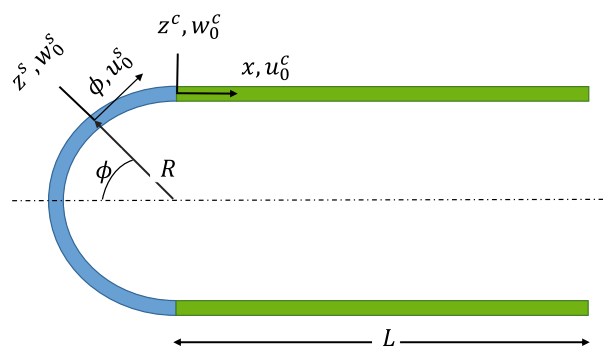
\includegraphics[width=0.75\textwidth]{vibro1_figure1.png}%
	\caption{Геометрические параметры и заданные системы координат объединенной цилиндрической и сферической оболочки}
	\label{fig:vibro1:1}
\end{figure}

\subsection{Описание свойств ФГМ} \label{ch:ch3/sec2/sub2}
Предполагается, что свойства материала керамической и металлической составляющих системы соединенных оболочек распределены по толщине на основе степенной функции. Предполагается, что объемная доля керамики \(V_c\) и объемная доля металла \(V_m\) подчиняются следующей форме [29-36*].

\begin{equation}
	\label{eq:vibro1:1}
	V_c = \left (\frac{1}{2}+\frac{z}{h} \right )^{k} ,\quad  V_m =1 - V_c
\end{equation}


В приведенном выше уравнении \(k\) является показателем функции и диктует распределение свойств материала по толщине. Очевидно, что поверхность \(z = +h/2\) богата керамикой, а поверхность \(z = -h/2\) богата металлом.


Следуя простому правилу подхода смесей (правило Фойгта), каждое свойство объединенной оболочки FG, например P, может быть записано как функция соответствующих свойств составляющих и объемной доли составляющих как

\begin{equation}
	\label{eq:vibro1:2}
	P(z) = P_m + P_{cm} \left (\frac{1}{2}+\frac{z}{h} \right )^{k} ,\quad  P_{cm} = P_c - P_m
\end{equation}

где \(P_m\) и \(P_c\) -- соответствующие свойства металлических и3 керамических компонентов, соответственно. В настоящей работе предполагается, что модуль упругости E и плотность массы \(\rho \) описываются уравнением (\cref{eq:vibro1:2}), а коэффициент Пуассона \(\mu \) считается постоянным по всей толщине, поскольку он изменяется только в небольшом диапазоне.


\subsection{Постановка задачи}\label{ch:ch3/sec2/sub3}

Рассмотрим объединенную цилиндрическо-полусферическую оболочку из функционально-градиентного материала равномерной толщины \(h\), радиуса сферы \(r^s = R\), радиуса цилиндра \(r^c = R\) и длины цилиндра \(L^c = L\). Система показана на \cref{fig:vibro1:1}. Система координат \((x, \theta, z)\) применяется к системе цилиндрической оболочки, а система \((\phi, \theta, z)\) -- к сферической оболочке. Системы координат также показаны на \cref{fig:vibro1:1}.

Чтобы учесть деформации сдвига по толщине и эффекты вращательной инерции цилиндрических и сферических оболочек, для формулировки определяющих уравнений оболочки используется теория сдвиговых деформаций первого порядка (\textbf{FSDT}) оболочек. На основе FSDT компоненты смещения в общей точке для цилиндрических и сферических оболочек могут быть представлены в соответствии с характеристиками средней поверхности таким образом, что

\begin{equation}
	\label{eq:vibro1:3}
	\begin{split}
	u^i (\xi, \theta, z, t) &= u_0^i(\xi, \theta, t)+ z \varphi_{\xi}^i (\xi, \theta,  t)\\
	v^i (\xi, \theta, z, t) &= v_0^i(\xi, \theta, t)+ z \varphi_{\theta}^i (\xi, \theta,  t)\\
	w^i (\xi, \theta, z, t) &= w_0^i (\xi, \theta, t)
	\end{split}
\end{equation}

В приведенном выше уравнении \(u, v, w\) -- это тангенциальное, окружное и поперечное перемещения по толщине, соответственно. Надстрочный индекс \(i\) может быть \(c\) или \(s\) для цилиндрических и сферических оболочек. Кроме того, \(\xi\) может принимать значение \(\phi\) или \(x\) для сферических и цилиндрических оболочек, соответственно. Подстрочный индекс 0 указывает на характеристики срединной поверхности. Кроме того, \(\phi_{\xi}\) и \(\phi_{\theta}\)  -- это, соответственно, повороты поперечных нормалей вокруг осей \(\theta\) и \(\xi\), соответственно.

Согласно FSDT, компоненты поля деформации в произвольной точке цилиндрической или сферической оболочки могут быть получены в терминах срединной поверхности оболочки и изменению кривизны.  Следовательно, можно записать [37*]

\begin{equation}
	\label{eq:vibro1:4}
	\begin{Bmatrix}
		\varepsilon_{\xi \xi}^i \\
		\varepsilon_{\theta \theta}^i \\
		\gamma_{\xi \theta}^i \\
		\gamma_{\xi z}^i \\
		\gamma_{\theta z}^i
	\end{Bmatrix} =
	\begin{Bmatrix}
		\varepsilon_{\xi \xi 0}^i \\
		\varepsilon_{\theta \theta 0}^i \\
		\gamma_{\xi \theta 0}^i \\
		\gamma_{\xi z 0}^i \\
		\gamma_{\theta z 0}^i
	\end{Bmatrix}
	+ z
		\begin{Bmatrix}
			\kappa_{\xi \xi}^i \\
			\kappa_{\theta \theta}^i \\
			\kappa_{\xi \theta}^i \\
			\kappa_{\xi z}^i \\
			\kappa_{\theta z}^i
	\end{Bmatrix}
\end{equation}

где компоненты деформации, связанные со средней поверхностью цилиндрической оболочки, имеют вид

\begin{equation}
\label{eq:vibro1:5}
\begin{Bmatrix}
		\varepsilon_{\xi \xi 0}^{c} \\
		\varepsilon_{\theta \theta 0}^{c} \\
		\gamma_{\xi \theta 0}^{c} \\
		\gamma_{\xi z 0}^{c} \\
		\gamma_{\theta z 0}^{c}
\end{Bmatrix} =
\begin{Bmatrix}
		u_{0, x}^c \\
		\frac{v_{0, \theta}^c}{r^c}+\frac{w_{0}^c}{r^c} \\
		\frac{u_{0, \theta}^c}{r^c}+v_{0, x}^c \\
		w_{0,x}^c+\varphi_{x}^c \\
		\frac{w_{0,\theta}^c}{r^c}-\frac{v_{0}^c}{r^c} + \varphi_{\theta}^c
\end{Bmatrix}
\end{equation}


и аналогично для сферической оболочки получаем

\begin{equation}
	\label{eq:vibro1:6}
	\begin{Bmatrix}
		\varepsilon_{\phi \phi 0}^{s} \\
		\varepsilon_{\theta \theta 0}^{s} \\
		\gamma_{\phi \theta 0}^{s} \\
		\gamma_{\phi z 0}^{s} \\
		\gamma_{\theta z 0}^{s}
	\end{Bmatrix} =
	\begin{Bmatrix}
		\frac{u_{0, \phi}^s}{r^s}+\frac{w_{0}^s}{r^s} \\
		\frac{v_{0, \theta}^s}{r^s \sin{\phi}}+\frac{u_{0}^s}{r^s} \cot{\phi}+\frac{w_0^s}{r^s} \\
		\frac{v_{0, \phi}^s}{r^s} +\frac{u_{0}^s}{r^s \sin{\phi}} -\frac{v_0^s}{r^s}\cot{\phi}\\
		\frac{w_{0, \phi}^s}{r^s} +\varphi_{\phi}^s -\frac{u_0^s}{r^s} \\
		\frac{w_{0,\theta}^c}{r^c}-\frac{v_{0}^c}{r^c} + \varphi_{\theta}^c
	\end{Bmatrix}
\end{equation}

Компоненты изменения кривизны в смысле Доннелла, совместимые с FSDT для цилиндрической оболочки [37*]

\begin{equation}
	\label{eq:vibro1:7}
	\begin{Bmatrix}
		\kappa_{xx}^{c} \\
		\kappa_{\theta \theta}^{c} \\
		\kappa_{x \theta}^{c} \\
		\kappa_{x z}^{c} \\
		\kappa_{\theta z}^{c}
	\end{Bmatrix} =
	\begin{Bmatrix}
		\varphi_{x,x}^c \\
		\frac{\varphi_{\theta, \theta}^c}{r^c} \\
		\frac{\varphi_{x, \theta}^c}{r^c}+\varphi_{\theta, x}^c \\
		0 \\
		0
	\end{Bmatrix}
\end{equation}

а для сферической оболочки могут быть записаны в виде

\begin{equation}
	\label{eq:vibro1:8}
	\begin{Bmatrix}
		\kappa_{\phi\phi}^{s} \\
		\kappa_{\theta \theta}^{s} \\
		\kappa_{\phi \theta}^{s} \\
		\kappa_{\phi z}^{s} \\
		\kappa_{\theta z}^{s}
	\end{Bmatrix} =
	\begin{pmatrix}
		\frac{\varphi_{\phi,\phi}^s}{r^s} \\
		\frac{\varphi_{\theta, \theta}^s}{r^s \sin{\phi}} + \frac{\varphi_{\theta}^s}{r^s}\cot{\phi} \\
		\frac{\varphi_{\theta, \phi}^s}{r^s}+\frac{\varphi_{\phi, \theta}^s}{r^s \sin{\phi}}-\frac{1}{r^s}\varphi_{\theta}^s \cot{\phi} \\
		0 \\
		0
	\end{pmatrix}
\end{equation}


Для случая, когда свойства материала оболочки линейно упругие, компоненты напряжения в виде деформаций рассчитываются как 

\begin{equation}
	\label{eq:vibro1:9}
	\begin{Bmatrix}
		\sigma_{\xi \xi}^i \\
		\sigma_{\theta \theta}^i \\
		\tau_{\xi \theta}^i \\
		\tau_{\xi z}^i \\
		\tau_{\theta z}^i
	\end{Bmatrix} =
	\begin{bmatrix}
		Q_{11} & Q_{12} & 0       & 0  	  & 0 \\
		Q_{12} & Q_{22} & 0       & 0     & 0 \\
		 0     &     0  & Q_{44}  & 0 	  & 0 \\
		 0     &     0  & 0       & Q_{55}& 0 \\
		 0     &     0  & 0       & 0     &  Q_{66}
	\end{bmatrix}
	\begin{Bmatrix}
		\varepsilon_{\xi \xi}^i \\
		\varepsilon_{\theta \theta}^i \\
		\gamma_{\xi \theta}^i \\
		\gamma_{\xi z}^i \\
		\gamma_{\theta z}^i
	\end{Bmatrix}
\end{equation}

где \(Q_{ij}, i,j =1, 2, 4, 5, 6\) являются приведенными коэффициентами жесткости материала и получаются следующим образом

\begin{equation}
	\label{eq:vibro1:10}
	Q_{11} = Q_{22} = \frac{E(z)}{1-\nu^2}, \quad Q_{12}=\frac{\nu E(z)}{1-\nu^2}, \quad Q_{44}=Q_{55}=Q_{66}=\frac{E(z)}{2(1+\nu)}
\end{equation}

Компоненты результирующих напряжений получены с использованием компонентов напряжений как [38*]

\begin{equation}
	\label{eq:vibro1:11}
	\begin{split}
	\begin{Bmatrix}
		N_{\xi \xi}^{i} \\
		N_{\theta \theta}^{i} \\
		N_{\xi \theta}^{i} 
	\end{Bmatrix} &=
	\int_{-h/2}^{+h/2}
	\begin{Bmatrix}
		\sigma_{\xi \xi}^{i} \\
		\sigma_{\theta \theta}^{i} \\
		\tau_{\xi \theta}^{i} 
	\end{Bmatrix}
	dz,\\
	\begin{Bmatrix}
	M_{\xi \xi}^{i} \\
	M_{\theta \theta}^{i} \\
	M_{\xi \theta}^{i} 
\end{Bmatrix} &=
\int_{-h/2}^{+h/2} z
\begin{Bmatrix}
	\sigma_{\xi \xi}^{i} \\
	\sigma_{\theta \theta}^{i} \\
	\tau_{\xi \theta}^{i} 
\end{Bmatrix}
dz,\\
	\begin{Bmatrix}
	Q_{\xi z}^{i} \\
	Q_{\theta z}^{i}
\end{Bmatrix} &=
\int_{-h/2}^{+h/2} k
\begin{Bmatrix}
	\tau_{\xi z}^{i} \\
	\tau_{\theta z}^{i}
\end{Bmatrix}
dz
\end{split}
\end{equation}

В приведенном выше уравнении \(k\) -- это поправочный коэффициент сдвига FSDT. Как известно, принятие поправочного коэффициента сдвига приводит к более точной оценке собственных частот. Поскольку поправочный коэффициент сдвига зависит от граничных условий, свойств материала и типа нагрузки [39*], точное его значение определить не просто. Однако широко используются приблизительные значения \(k = 5/6 \) или \(k = \pi^2 / 12\). В данном исследовании коэффициент коррекции сдвига равен \(k = 5/6 \).


Подстановка \cref{eq:vibro1:11} в уравнение \cref{eq:vibro1:11} с одновременным использованием уравнений \cref{eq:vibro1:4}-\cref{eq:vibro1:8} дает результирующие напряжения в виде характеристик средней поверхности оболочки в виде

\begin{equation}
	\label{eq:vibro1:12}
	\begin{Bmatrix}
		N_{\xi \xi}^{i}\\
		N_{\theta \theta}^{i} \\
		N_{\xi \theta}^{i} \\
		M_{\xi \xi}^{i} \\
		M_{\theta \theta}^{i}\\
		M_{\xi \theta}^{i}\\
		Q_{\xi z}^{i}\\
		Q_{\theta z}^{i}	
	\end{Bmatrix} =
\begin{bmatrix}
	A_{11} & A_{12} & 0 & B_{11} & B_{12} & 0 & 0 & 0 \\
	A_{12} & A_{22} & 0 & B_{12} & B_{22} & 0 & 0 & 0 \\
	0 & 0 & A_{66} & 0 & 0 & 0 & 0 & 0 \\
	B_{11} & B_{12} & 0 & D_{11} & D_{12} & 0 & 0 & 0 \\
	B_{12} & B_{22} & 0 & D_{12} & D_{22} & 0 & 0 & 0 \\
	0 & 0 & 0 & 0 & 0 & D_{66} & 0 & 0 \\
	0 & 0 & 0 & 0 & 0 & 0 & k A_{44} & 0 \\
	0 & 0 & 0 & 0 & 0 & 0 & 0 & k A_{55}
\end{bmatrix}
	\begin{Bmatrix}
		\varepsilon_{\xi \xi 0}^{i}\\
		\varepsilon_{\theta \theta 0}^{i} \\
		\gamma_{\xi \theta 0}^{i} \\
		\kappa_{\xi \xi }^{i} \\
		\kappa_{\theta \theta}^{i}\\
		\kappa_{\xi \theta}^{i}\\
		\gamma_{\xi z 0}^{i}\\
		\gamma_{\theta z 0}^{i}
	\end{Bmatrix}
\end{equation}

В приведенном выше уравнении постоянные коэффициенты \(A_{i j} , B_{i j} и D_{i j}\) обозначают известные жесткости на растяжение, каплинга и изгиба, соответственно, которые рассчитываются по формуле

\begin{equation}
	\label{eq:vibro1:13}
	\left ( A_{i j} , B_{i j} и D_{i j} \right ) = \int_{-0.5 h}^{+0.5h} \left ( Q_{i j} , zQ_{i j} , z^2 Q_{i j} \right ) dz
\end{equation}

Полный набор уравнений движения и граничных условий объединенной системы цилиндрических и полусферических оболочек может быть получен на основе обобщенного принципа Гамильтона [38*]. Утверждение принципа Гамильтона гласит

\begin{equation}
	\label{eq:vibro1:14}
	\begin{split}
	\delta \int_{t_1}^{t_2} \left (K^i - \left ( U^i +V^i \right ) \right )\,dt = 0 \\
	\text{at } t=t_1,t_2: \delta u_0^i= \delta v_0^i=\delta w_0^i=\delta \varphi_{\xi}^i= \delta \varphi_{\theta}^i=0
	\end{split}
\end{equation}

где в приведенном выше уравнении \(\delta K^i\) -- виртуальная кинетическая энергия цилиндрической/сферической оболочки, которая равна

\begin{equation}
	\label{eq:vibro1:15}
	\delta K^i = \int_V^i \rho (z) \left ( \dot{u}^i \delta \dot{u}^i + \dot{v}^i \delta \dot{v}^i + \dot{w}^i \delta \dot{w}^i \right )\, dV^i
\end{equation} 
Тут точкой обозначена проихводная по времени. Поскольку \(\delta U^i\) виртуальная энергия деформации для цилиндрической/сферической оболочки, которая записывается следующим образом

\begin{equation}
	\label{eq:vibro1:16}
	\delta U^i = \int_V^i \left ( \sigma_{\xi \xi}^i \delta \varepsilon_{\xi \xi}^i + \sigma_{\theta \theta}^i \delta \varepsilon_{\theta \theta}^i +  \tau_{\xi \theta}^i \delta \gamma_{\xi \theta}^i + \kappa \tau_{\theta z}^i \delta \gamma_{\theta z}^i + \kappa \tau_{\xi z}^i \delta \gamma_{\xi z}^i \right ) \, dV^i
\end{equation}

А \(\delta V^i \) -- виртуальная потенциальная энергия внешних нагрузок, которая отсутствует для задачи свободных колебаний. Интегрирование вышеприведенных выражений по координате \(z\) и применение теоремы Грина-Гаусса для освобождения виртуальных градиентов перемещений приводит к выражениям для линейных уравнений движения цилиндрической и сферической оболочек, соответственно, в виде

\begin{equation}
	\label{eq:vibro1:17}
	\begin{split}
	N_{xx,x}^c &+ \frac{N_{x \theta,\theta}^c}{R} = I_1 \ddot{u}_0^i+I_2 \ddot{\varphi}_x^c
	\\
	\frac{N_{\theta \theta,\theta}^c}{R} &+ N_{x \theta,x}^c + \frac{Q_{\theta z}^c}{R} = I_1 \ddot{v}_0^i+I_2 \ddot{\varphi}_{\theta}^c
	\\
	Q_{xz,x}^c &+ \frac{Q_{\theta z,\theta}^c}{R} - \frac{N_{\theta \theta}^c}{R} = I_1 \ddot{w}_0^c
	\\
	M_{xx,x}^c &+ \frac{M_{x \theta, \theta}^c}{R} - Q_{xz}^c = I_2 \ddot{u}_0^c + I_3 \ddot{\varphi}_x^c
	\\
	M_{x \theta,x}^c &+ \frac{M_{\theta \theta, \theta}^c}{R} - Q_{\theta z}^c = I_2 \ddot{v}_0^c + I_3 \ddot{\varphi}_{\theta}^c
	\end{split}
\end{equation} 


\begin{equation}
	\label{eq:vibro1:18}
	\begin{split}
		\frac{N_{\phi \phi, \phi}^s}{R} &+ \frac{N_{\phi \theta,\theta}^s}{R\sin{\phi}} + \frac{N_{\phi \phi}^s - N_{\theta \theta}^s}{R} \cot{\phi} + \frac{Q_{\phi}}{r}= I_1 \ddot{u}_0^i+I_2 \ddot{\varphi}_x^c
		\\
		\frac{N_{\theta \theta, \theta}^s}{R \sin{\phi}} &+ \frac{N_{\phi \theta,\phi}^s}{R} + 2\frac{\cot{\phi}}{R} N_{\phi \theta}^s + \frac{Q_{\theta}^s}{R}= I_1 \ddot{v}_0^i+I_2 \ddot{\varphi}_{\theta}^c
		\\
		\frac{Q_{\phi z, \phi}^s}{R} &+ \frac{1}{R \sin{\phi}} Q_{\theta, \theta}^s + \frac{Q_{\phi}^s}{R}\cot{\phi}  - \frac{N_{\phi \phi}^s + N_{\theta \theta}^s}{R} = I_1 \ddot{w}_0^s
		\\
		\frac{M_{\phi \phi, \phi}^s}{R}&+\frac{M_{\phi \theta, \theta}^s}{R \sin{\phi}}+\frac{M_{\phi \phi}^s - M_{\theta \theta}^s}{R} \cot{\phi} - Q_{\phi}^s =I_2 \ddot{u}_0^s + I_3 \ddot{\varphi}_{\phi}^s
		\\
		\frac{M_{\theta \theta, \theta}^s}{R \sin{\phi}}&+\frac{M_{\phi \theta, \phi}^s}{R }+2\frac{\cot{\phi}}{R} M_{\phi \theta}^s - Q_{\phi}^s =I_2 \ddot{v}_0^s + I_3 \ddot{\varphi}_{\theta}^s
	\end{split}
\end{equation} 

В \cref{eq:vibro1:18} обозначение \(R\) используется как для \(r^c\), так и для \(r^s\). Также применяются следующие определения. В \cref{eq:vibro1:18} обозначение \(R\) используется как для \(r^c\), так и для \(r^s\). Кроме того, применяются следующие определения

\begin{equation}
	\label{eq:vibro1:19}
	\left ( I_1, I_2, I_3 \right ) = \int_{-h/2}^{+h/2} \rho (1, z, z^2)\, dz
\end{equation}

Для конца цилиндрической оболочки могут быть определены различные типы граничных условий. Край \(x = L\) может быть зажатым (C) или свободным (F). 


\subsection{Алгоритм поиска решения}\label{ch:ch3/sec2/sub4}

Ссылаясь на определения нормальной силы и изгибающего момента из уравнения \cref{eq:vibro1:12} и уравнений движения \cref{eq:vibro1:17} и \cref{eq:vibro1:18}, следующее разделение переменных точно удовлетворяет условиям периодичности полевых переменных, а также совместимо с уравнениями движения \cref{eq:vibro1:17} и \cref{eq:vibro1:18} и условиями соответствия \cref{eq:vibro1:22} и \cref{eq:vibro1:23}.

\begin{equation}
	\label{eq:vibro1:24}
	\begin{Bmatrix}
		u_0^i(\xi, \theta, t) \\
		v_0^i(\xi, \theta, t) \\
		w_0^i(\xi, \theta, t) \\
		\varphi_{\xi}^i(\xi, \theta, t) \\
		\varphi_{\theta}^i(\xi, \theta, t)
	\end{Bmatrix} =
	\cos({\omega t + \psi})
\begin{bmatrix}
	\sin{n \theta} & 0 & 0 & 0 & 0 \\
	0 & \cos{n \theta} & 0 & 0 & 0 \\
	0 & 0 & \sin{n \theta} & 0 & 0 \\
	0 & 0 & 0 & \sin{n \theta} & 0 \\
	0 & 0 & 0 & 0 & \cos{n \theta}
\end{bmatrix}
	\begin{Bmatrix}
		U^i(\xi) \\
		V^i(\xi) \\
		W^i(\xi) \\
		\Phi_{\xi}^i(\xi) \\
		\Phi_{\theta}^i(\xi)
	\end{Bmatrix}
\end{equation}

где в приведенном выше уравнении \(n\), как уже упоминалось, является волновым числом в окружном направлении. Временная зависимость решения \cref{eq:vibro1:24} выбрана для преодоления условия периодичности поля переменных во временной области. В этой функции \(\omega\) -- собственная частота объединенной системы оболочек.


Подстановка вышеприведенного уравнения в уравнения движения \cref{eq:vibro1:17} и \cref{eq:vibro1:18} приводит к новым десяти связанным обыкновенным дифференциальным уравнениям в терминах неизвестных сквозных меридианных функций \(U^i(\xi), V^i(\xi), W^i (\xi), \Phi_{\xi}^i, \Phi_{\theta}^i\). Преобразованные уравнения и соответствующие граничные условия для цилиндрического/сферического сегмента здесь не приводятся и представлены в "Приложении A".

Как и ожидалось, уравнения (A.1)-(A.10) вместе с правильным выбором граничных и согласующих условий приводят к системе однородных уравнений. Чтобы решить систему уравнений как задачу на собственные значения, применяется метод GDQ для преобразования обыкновенных дифференциальных уравнений (A.1)-(A.10) в новые линейные алгебраические уравнения. Метод GDQ достаточно хорошо известен, и его детали здесь не повторяются. Между тем, за более подробной информацией можно обратиться к [41*]. Стоит отметить, что распределение узловых точек в каждом сегменте описывается с помощью точек Чебышева-Гаусса-Лобатто, что приводит к следующим результатам

Известны четыре общие процедуры для наложения граничных условий на дискретизированную систему на основе GDQ. В данном исследовании для применения граничных и согласующих условий используется метод SBCGE, который непосредственно подставляет граничные условия в управляющие уравнения. Основываясь на этой технике, необходимо применить метод GDQ как к уравнениям движения, так и к граничным условиям. Уравнения движения после дискретизации, применения согласующих и граничных условий и глобальной ассемблировки принимают вид

\begin{equation}
\label{eq:vibro1:26}
\boldsymbol{K } \Delta = \omega^2 \boldsymbol{M} \Delta
\end{equation}

где в приведенном выше уравнении \(M\) -- обобщенная матрица масс, \(K\) -- обобщенная матрица жесткости и неизвестный вектор перемещения. Собственные частоты конструкции могут быть получены путем решения стандартной задачи на собственные значения \cref{eq:vibro1:26}.

\subsection{Вывод для данного решения}\label{ch:ch3/sec2/sub5}

 данном исследовании оценивается отклик свободных колебаний объединенной системы цилиндрической и полусферической оболочек. Предполагается, что оболочка изготовлена из FGM, свойства которого градируются в направлении толщины. Для описания объемной доли компонентов используется простая функция степенного закона, а для оценки свойств применяется простое правило смесей Фойгта. Для создания управляющих уравнений системы оболочек используется теория оболочек сдвиговой деформации первого порядка и кинематические предположения типа Доннелла. Используя принцип Гамильтона, получен полный набор управляющих уравнений и граничных условий для оболочек. С помощью разложения Фурье по окружности и метода GDQ для управляющих уравнений, граничных условий и условий согласования пересечений получена полная система алгебраических уравнений, которая решается как задача с собственными значениями. После проверки результатов данного исследования для случая однородных оболочек, получены новые численные результаты для случая оболочек FGM. Показано, что индекс силового закона FGM, отношение радиуса к длине цилиндрической оболочки и отношение длины к радиусу являются важными факторами, влияющими на частоты объединенной системы оболочек.
 
\section{Автоколебания пластины из ФГМ под действием быстрого нагрева} \label{ch:ch3/sec3}

\subsection{Обзор}\label{ch:ch3/sec3/sub1}
В данной части работы анализируется термоиндуцированная вибрация кольцевой секторной пластины из функционально-градиентных материалов. Считается, что все термомеханические свойства среды FGM зависят от температуры. На основе теории линейной термоупругости без связи устанавливается одномерное переходное уравнение теплопроводности типа Фурье. Верхняя и нижняя поверхности пластины находятся под различными типами граничных условий быстрого нагрева. Из-за зависимости свойств материала от температуры уравнение теплопроводности становится нелинейным. Поэтому необходимо использовать численный метод. Сначала для дискретизации уравнения теплопроводности по толщине пластины применяется метод обобщенных дифференциальных квадратур (\textbf{GDQM}). Затем, управляющая система зависящих от времени обыкновенных дифференциальных уравнений решается с помощью метода последовательного марширования по времени Крэнка-Николсона. Полученные результирующие тепловой силы и теплового момента на каждом временном шаге от температурного профиля применяются к уравнениям движения. Уравнения движения, основанные на теории деформации сдвига первого порядка (\textbf{FSDT}), получены с помощью принципа Гамильтона. С помощью GDQM двумерная область секторной пластины и подходящих граничных условий разбивается на ряд узловых точек, а дифференциальные уравнения превращаются в систему обыкновенных дифференциальных уравнений. Для получения неизвестного вектора смещения в любой момент времени используется метод прямого интегрирования, основанный на маршевой схеме Ньюмарка по времени. Для проверки формулировки и метода решения в настоящем исследовании проводятся сравнительные исследования. На различных примерах рассматривается влияние таких эффективных параметров, как показатель степени в зависимости FGM, толщина пластины, зависимость от температуры, угол раскрытия сектора, значения радиуса, граничные условия в плоскости и тип граничных условий быстрого нагрева на термоиндуцированный отклик пластины FGM при тепловом ударе.


Исследования термоиндуцированного отклика тонких конструктивных элементов в основном можно разделить на квазистатические и динамические исследования. Первые работы по теме термоиндуцированных колебаний принадлежат Болею [1**, 2**]. Болей [1**] исследовал динамический отклик быстро нагретой изотропной тонкой балки. В этом исследовании результаты показали, что параметр инерции, который зависит от геометрии и термомеханических свойств, является основным фактором. Боли и Барбер [2**] также проанализировали быстрый нагрев прямоугольных просто поддерживаемых пластин. Аналитические ряды Фурье используются для получения отклика пластины. Краус [3**] исследовал термоиндуцированную вибрацию сферических оболочек. Предполагается, что оболочка находится под тепловым ударом на одной поверхности, в то время как другая поверхность теплоизолирована. Он подтвердил важность параметра инерции для вибрационного поведения тонких оболочек при тепловом ударе.  Другим основным результатом его исследования является то, что из-за связи растяжения-изгиба в кинематике оболочек, параметр инерции в балках играет более определяющую роль, чем в пластинах и оболочках, соответственно. Страуд и Майерс [4**] использовали модифицированный вариационный принцип энергии Рейсса для изучения влияния зависимости от температуры на термоиндуцированные колебания пластин, подвергнутых произвольному тепловому удару. Исходя из полученных результатов, игнорирование температурной зависимости свойств материала приводит к ошибочным результатам в термоиндуцированной реакции пластин при тепловом ударе.


Осесимметричный динамический прогиб круглых пластин при быстром нагреве рассмотрен Накаджо и Хаяши [5**]. Они исследовали термоиндуцированную вибрацию на основе экспериментальных, аналитических и численных методов, используя линейные и нелинейные соотношения деформации и перемещения. Как было замечено в этом исследовании, для специальных граничных условий, основанных на линейной теории, пластина демонстрирует различные реакции, полученные экспериментальным и теоретическим методами. Киани и Эслами [6**] проанализировали нелинейную термоиндуцированную вибрацию функционально-градиентных круглых пластин на основе геометрической нелинейности типа фон Кармана. Предполагается, что термоупругие свойства материала зависят от температуры. Они сообщили, что конструкции без начальной кривизны с зажатыми краями способны компенсировать дополнительные моменты для сохранения прямолинейного состояния до определенного времени, в течение которого наступает динамическая неустойчивость и конструкция вибрирует. Эслами [7**] в учебнике проанализировал нелинейную динамическую тепловую неустойчивость различных типов тонких структур на основе нескольких методов.


В работе Venkataramana и Jana [8**] анализируется быстрый нагрев изотропной балки, подверженной гармоническому изменению температуры. Отклик балки получен в двух частях: статической и динамической. В вышеупомянутом исследовании, основанном на процедуре суперпозиции, полный прогиб имеет тенденцию колебаться вокруг статической реакции. Кидава-Кукла [9**] использовал схему функции Грина для обсуждения вынужденных колебаний балок, подверженных воздействию движущегося концентрированного источника тепла. В этом исследовании рассматриваются эффекты внутреннего и внешнего демпфирования на поперечный отклик. Брух и др. [10**] разработали стратегию активного управления для уменьшения максимальной деформации и скорости просто поддерживаемой быстро нагреваемой балки.  Влияние сжимающих нагрузок в плоскости и внутреннего/внешнего демпфирования на тепловые прогибы балочных конструкций описано Манолисом и Бескосом [11**]. Решение уравнения колебательного движения во временной области получено с помощью метода численного преобразования Лапласа. Адам и др. [12**] исследовали эффект межслойного скольжения на тепловой отклик вязкоупругих композитных балок Эйлера-Бернулли. Разделив динамическую реакцию на квазистатическую и дополнительную динамическую части, получена реакция балки при быстром нагреве. Квазистатическое решение определено в замкнутой форме, а оставшаяся дополнительная динамическая часть получена численно с помощью усеченного модального ряда. Явление теплового флаттера изотропных консольных балок при солнечном нагреве проанализировано Чжаном и другими [13**]. Они ввели критерий, согласно которому тепловой флаттер может возникнуть, если угол распространения солнечного теплового потока меньше угла изгиба свободного края, когда балка находится в квазистатическом равновесии. Малик и Кадоли [14**] исследовали термоиндуцированную вибрацию балок из FGM при различных типах быстрого нагрева. Предполагается, что одна поверхность балки подвергается воздействию движущейся нагревательной нагрузки, ступенчатого нагрева, ударного нагрева и сосредоточенного линейного источника тепла, а противоположная поверхность термически изолирована или подвергается конвективным потерям тепла. Основываясь на методе Ритца и используя теорию деформации сдвига первого порядка, Гиасян и др. [15**] исследовали нелинейный тепловой прогиб быстро нагреваемой балки ФГМ. Все свойства материала считаются зависящими от температуры


Таухерт [16**] исследовал термоиндуцированную вибрацию ортотропных прямоугольных пластин с различными типами граничных условий, связанных с краевыми опорами типа Леви.  Применяя метод комплексных переменных к уравнениям движения, Дас [17**] проанализировал термоиндуцированную реакцию пластин произвольной многоугольной формы, подвергнутых тепловому удару.  Влияние пьезо-термоупругих слоев на подавление реакции прямоугольных и круглых пластин при тепловом ударе исследовано Таухертом и др [18**]. Чанг и др. [19**] провели исследование для получения отклика быстроударных слоистых композитных пластин с использованием двумерного вариационного метода конечных элементов. Для аппроксимации полей перемещений используется теория высшего порядка, учитывающая поперечные сдвиговые и нормальные деформации. Алипур и др. [20**] исследовали термоиндуцированную реакцию квадратных пластин с учетом положения и зависящих от температуры свойств материала. Для дискретизации уравнений движения применяется двумерный обобщенный дифференциальный квадратичный метод.  С помощью хорошо известного метода Рунге-Кутты четвертого порядка был получен отклик пластины. Джавани и др. исследовали геометрически нелинейный тепловой прогиб кольцевой пластины ФГМ [21**], неглубоких арок [22**], сферических оболочек [23**] и конических оболочек [24**] с зависящими от температуры свойствами материала, используя метод дифференциальных квадратур.


Хилл и Мазумдар [25**] предложили методику для теплового прогиба вязкоупругих пластин и тонких оболочек, испытывающих большие прогибы. Метод решения в основном заимствован из предыдущих исследований авторов для типа связей деформация-перемещение [26-28**]. Однако методология решения может быть применима даже для прогибов, которые находятся в диапазоне толщины конструкции. Быстро нагревающиеся поперечные слоистые трубы исследованы на основе двумерного метода GDQ Хонгом и другими [29**]. Esmaeili и др. [30**] представили осесимметричные термоиндуцированные колебания большой амплитуды цилиндрических оболочек из материала FG, зависящего от температуры, используя метод Ритца. Хуанг и Таухерт [31**] исследовали быстрый нагрев композитных панелей. Решение Навье применяется для получения теплового прогиба просто поддерживаемых поперечных симметричных и антисимметричных ламинированных панелей двойной кривизны.  Геометрически нелинейные деформации цилиндрических панелей с использованием теории фон Кармана при тепловых ударах исследованы Хуангом и Таухертом [32**]. В этом исследовании используется двумерный метод конечных элементов. Кейболахи и др. [33**] продемонстрировали, что при некоторых особых геометрических и граничных условиях динамическое термическое смятие тонких шалевых арок происходит при термоиндуцированной вибрации. Используя метод Ритца и критерий Будянского-Хатчинсона, была получена критическая температура. Кейболахи и др. [34**] развили предыдущую работу для анализа нелинейного быстрого нагрева неглубоких арок с различными типами граничных условий. Основываясь на классической теории оболочек, Хдейр [35**, 36**] сообщил о термоиндуцированной реакции неглубоких оболочек и арок, подверженных быстрому нагреву, используя аналитический метод.  Путем внедрения связанной и несвязанной теорий термовязкости в уравнения движения быстро нагружаемых толстых круговых цилиндрических слоистых композитных оболочек Чанг и Шьонг [37**] проанализировали тепловую реакцию с помощью метода конечных элементов. Управление тепловым прогибом в пьезо-гигро-термоупругих слоистых пластинах и оболочках выполнено Раджа и др [38**]. Также Кумар и др. [39] исследовали вынужденные колебания пьезо-ламинированных тонких цилиндрических оболочек под электрическими, механическими и тепловыми нагрузками с помощью метода конечных элементов.  Пандей и Прадьюмна [40**] проанализировали многослойные пластины FGM и двояковогнутые панели при быстром нагреве.  В данном исследовании рассматривается теория слоев высшего порядка.


В настоящем исследовании впервые исследуется термоиндуцированная вибрация зависящей от температуры кольцевой секторной пластины из ФГМ с произвольными граничными условиями. Предполагается, что термомеханические свойства пластины зависят от температуры. Нелинейное уравнение теплопроводности типа Фурье с граничными условиями быстрого нагрева в верхней и боковой плоскостях решается одномерным обобщенным методом квадратурных разностей (\textbf{GDQM}) и маршевой схемой Кранка-Никольсона. С помощью теории сдвиговой деформации пластин первого порядка и двумерного GDQM получены матрицы упругой жесткости и массы, а также вектор силы секторной пластины. Система зависящих от времени обыкновенных дифференциальных уравнений решается с помощью гибридного метода Ньюмарка-Ньютона-Рафсона для получения профиля бокового прогиба секторной пластины во временной области. Сравнительное исследование позволяет убедиться в эффективности и точности разработанной методики. Представлено влияние различных параметров на термоиндуцированный прогиб быстроударной кольцевой секторной пластины.


\subsection{Модель материала пластины}\label{ch:ch3/sec3/sub2}

\begin{figure}[h!]
	\centering
	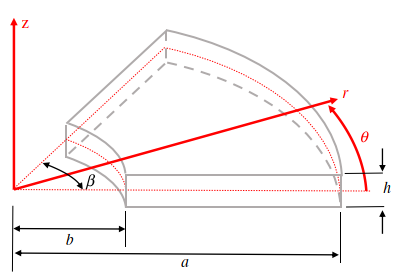
\includegraphics[width=0.75\textwidth]{vibro2_figure1.png}%
	\caption{Схема и локальная СК для сектора из ФГМ}
	\label{fig:vibro2:1}
\end{figure}

Рассмотрим металлокерамическую функционально-градиентную кольцевую секторную пластину внутреннего радиуса \(b\), внешнего радиуса \(a\) и толщины \(h\). Как показано на \cref{fig:vibro2:1}, задана система полярных координат \((r, \theta, z\)) с началом координат в центре средней плоскости секторной пластины.  Как обычно, \((r, \theta, z\)) показывают радиальное, окружное и поперечное направления, соответственно.


Эффективные термомеханические свойства кольцевой секторной пластины FGM могут быть определены в соответствии с надлежащей процедурой гомогенизации. Правило смеси Войгта обычно используется из-за его простоты и эффективности [41**-48**]. Согласно этому правилу, механические и тепловые характеристики пластины FGM, такие как модуль Юнга \(E\),  \(\nu\)коэффициент Пуассона, \(\alpha\)коэффициент теплового расширения, \(\rho\) массовая плотность, удельная теплоемкость \(C_v\) и теплопроводность \(K\), считаются линейными функциями объемных долей керамики \(V_c\) и металла \(V_m\). Таким образом, как функция направления толщины, неоднородное свойство пластины, \(P\), может быть выражено в виде [49**]

\begin{equation}
	\label{eq:vibro2:1}
	\begin{split}
	P(z, T) &= P_m(T) + V_c (z) P_{cm}(T)\\
	P_{cm}(T) &= P_c(T) - P_m(T)
	\end{split}
\end{equation}

Температурная зависимость составляющих ФГМ часто выражается на основе формулы Тулукиана. Соответственно, каждое свойство металла или керамики может быть записано в форме [49**]

\begin{equation}
	\label{eq:vibro2:2}
		P(T) = P_0 \left (P_{-1}T^{-1}+1+P_1 T^1 + P_2 T^2 + P_3 T^3 \right )
\end{equation}

В котором \(T\) -- температура, измеренная в Кельвинах, а \(P^i\) -- константы, уникальные для каждого компонента. Придерживаясь обозначений Редди и Чину [49**], для представления объемной доли керамики \(V_c\) и объемной доли металла \(V_m\) можно использовать распределение по степенному закону в направлении толщины так, что

\begin{equation}
	\label{eq:vibro2:3}
	V_c = \left ( \frac{1}{2} + \frac{z}{h} \right ) ^{\xi}, \quad V_m = 1 - V_c
\end{equation}
Здесь \(\xi\) -- неотрицательный показательстепени, определяющий профиль дисперсии свойств.

\subsection{Постановка задачи}\label{ch:ch3/sec3/sub3}

Численные результаты данного исследования ограничиваются оценкой бокового прогиба на основе теории сдвиговых деформаций первого порядка (\textbf{FSDT}). Согласно двумерной FSDT, смещения общей точки секторной пластины характеризуются в терминах смещений средней поверхности как:

\begin{equation}
	\label{eq:vibro2:4}
	\begin{split}
		u^i (r, \theta, z, t) &= u_0^i(r, \theta, t)+ z \varphi_{r}^i (r, \theta,  t)\\
		v^i (r, \theta, z, t) &= v_0^i(r, \theta, t)+ z \varphi_{\theta}^i (r, \theta,  t)\\
		w^i (r, \theta, z, t) &= w_0^i (r, \theta, t)
	\end{split}
\end{equation}
где \(u, v, w\)) -- перемещение срединной поверхности в трех направлениях. \( \varphi_{r}, \varphi_{\theta} \) -- обозначают продольные вращения вокруг осей \( \theta, r\).


Компоненты деформации, связанные с полями перемещений \cref{eq:vibro2:4}, согласно теории кольцевых секторных пластин, могут быть представлены в виде:

\begin{equation}
	\label{eq:vibro1:5}
	\begin{split}
		\varepsilon_{rr} &= u_{0, r}
		\\
		\varepsilon_{\theta \theta } &= \frac{u}{r}+\frac{v{,\theta}}{r}
		\\
		\gamma_{r \theta} &= \frac{u_{, \theta}}{r}+v_{, r} - \frac{1}{r}v
		\\
		\gamma_{r z } &= u_{,z}+w_{,r}
		\\
		\gamma_{\theta z} &= v_{,z}-\frac{1}{r} w_{,\theta} 
	\end{split}
\end{equation}

где эпсилон это соответсвующее перемещение, а гамма это сдвиг. Запятая обозначает производную.

Рассматриваем \(T \)и \(T_0\) как распределение температуры и температуру начала отсчета и предполагая линейный термоупругий материал (закон Гука), определяющий закон для секториальной пластины ФГМ, подверженной тепловым нагрузкам, имеет вид

\begin{equation}
	\label{eq:vibro2:6}
	\begin{Bmatrix}
		\sigma_{\xi \xi}^i \\
		\sigma_{\theta \theta}^i \\
		\tau_{\xi \theta}^i \\
		\tau_{\xi z}^i \\
		\tau_{\theta z}^i
	\end{Bmatrix} =
	\begin{bmatrix}
		Q_{11} & Q_{12} & 0       & 0  	  & 0 \\
		Q_{12} & Q_{22} & 0       & 0     & 0 \\
		0     &     0  & Q_{44}  & 0 	  & 0 \\
		0     &     0  & 0       & Q_{55}& 0 \\
		0     &     0  & 0       & 0     &  Q_{66}
	\end{bmatrix}
	\left (
	\begin{Bmatrix}
		\varepsilon_{\xi \xi}^i \\
		\varepsilon_{\theta \theta}^i \\
		\gamma_{\xi \theta}^i \\
		\gamma_{\xi z}^i \\
		\gamma_{\theta z}^i
	\end{Bmatrix}
	- (T-T_0))
		\begin{Bmatrix}
		\alpha \\
		\alpha \\
		0 \\
		0 \\
		0
	\end{Bmatrix}
	\right )
\end{equation}

где \(Q_{ij}, i,j =1, 2, 4, 5, 6\) являются приведенными коэффициентами жесткости материала и получаются следующим образом

\begin{equation}
	\label{eq:vibro2:7}
	\begin{split}
	Q_{11} = Q_{22} &= \frac{E(z, T)}{1-\nu^2(z, T)}, \quad Q_{12}=\frac{\nu(z, T) E(z, T)}{1-\nu^2(z,T)}
	\\
	Q_{66}&=\frac{E(z, T)}{2(1+\nu(z, T))} \quad Q_{44}=Q_{55}=kQ_{66}
	\end{split}
\end{equation}
где \(k=5/6\) как было выбрано ранее.

Используя FSDT, результирующие напряжения мембраны \(N_{rr}, N_{\theta \theta}, и N_{r \theta}\), результирующие напряжения сдвига вне плоскости мембраны\( Q_r , Q_{\theta},\) и результирующие напряжения изгиба \(M_{rr}, M_{\theta, \theta}, M_{r \theta}\) могут быть представлены при интегрировании компонентов напряжения как


\begin{equation}
	\label{eq:vibro2:8}
	\begin{split}
		\begin{Bmatrix}
			N_{r r}^{i} \\
			N_{\theta \theta}^{i} \\
			N_{ \theta}^{i} 
		\end{Bmatrix} &=
		\int_{-h/2}^{+h/2}
		\begin{Bmatrix}
			\sigma_{r \xi}^{i} \\
			\sigma_{\theta \theta}^{i} \\
			\tau_{r \theta}^{i} 
		\end{Bmatrix}
		dz,\\
		\begin{Bmatrix}
			M_{rr}^{i} \\
			M_{\theta \theta}^{i} \\
			M_{r \theta}^{i} 
		\end{Bmatrix} &=
		\int_{-h/2}^{+h/2} z
		\begin{Bmatrix}
			\sigma_{rr}^{i} \\
			\sigma_{\theta \theta}^{i} \\
			\tau_{r \theta}^{i} 
		\end{Bmatrix}
		dz,\\
		\begin{Bmatrix}
			Q_{r}^{i} \\
			Q_{\theta}^{i}
		\end{Bmatrix} &=
		\int_{-h/2}^{+h/2} k
		\begin{Bmatrix}
			\tau_{r z}^{i} \\
			\tau_{\theta z}^{i}
		\end{Bmatrix}
		dz
	\end{split}
\end{equation}

Подставляя \cref{eq:vibro2:6} в \cref{eq:vibro2:8} с помощью уравнений \cref{eq:vibro2:4} и \cref{eq:vibro2:5}, результирующие напряжения в компонентах смещения получаются как \cref{eq:vibro1:12} с учетом еще одного члена.

\begin{equation}
	\label{eq:vibro2:9}
	\begin{Bmatrix}
		N_{\xi \xi}^{i}\\
		N_{\theta \theta}^{i} \\
		N_{\xi \theta}^{i} \\
		M_{\xi \xi}^{i} \\
		M_{\theta \theta}^{i}\\
		M_{\xi \theta}^{i}\\
		Q_{\xi z}^{i}\\
		Q_{\theta z}^{i}	
	\end{Bmatrix} =
	-
		\begin{Bmatrix}
		N^{T}\\
		N^{T} \\
		0\\
		M^{T}\\
		M^{T}\\
		0\\
		0\\
		0	
	\end{Bmatrix}
	+
	\begin{bmatrix}
		A_{11} & A_{12} & 0 & B_{11} & B_{12} & 0 & 0 & 0 \\
		A_{12} & A_{22} & 0 & B_{12} & B_{22} & 0 & 0 & 0 \\
		0 & 0 & A_{66} & 0 & 0 & 0 & 0 & 0 \\
		B_{11} & B_{12} & 0 & D_{11} & D_{12} & 0 & 0 & 0 \\
		B_{12} & B_{22} & 0 & D_{12} & D_{22} & 0 & 0 & 0 \\
		0 & 0 & 0 & 0 & 0 & D_{66} & 0 & 0 \\
		0 & 0 & 0 & 0 & 0 & 0 & k A_{55} & 0 \\
		0 & 0 & 0 & 0 & 0 & 0 & 0 & k A_{55}
	\end{bmatrix}
	\begin{Bmatrix}
		\varepsilon_{rr}^{i}\\
		\varepsilon_{\theta \theta} \\
		\gamma_{r \theta} \\
		\kappa_{r r} \\
		\kappa_{\theta \theta}\\
		\kappa_{r \theta}\\
		\gamma_{r z }\\
		\gamma_{\theta z}
	\end{Bmatrix}
\end{equation}


В приведенном выше уравнении постоянные коэффициенты \(A_{i j} , B_{i j} и D_{i j}\) обозначают известные жесткости на растяжение, каплинга и изгиба, соответственно, которые рассчитываются по формуле \cref{eq:vibro1:13}

\begin{equation}
	\label{eq:vibro2:10}
	\left ( A_{i j} , B_{i j} и D_{i j} \right ) = \int_{-0.5 h}^{+0.5h} \left ( Q_{i j} , zQ_{i j} , z^2 Q_{i j} \right ) dz
\end{equation}

Кроме этого термальные погонные силы и моменты расчитываются по формуле

\begin{equation}
	\label{eq:vibro2:11}
	\left ( N^T, M^T \right ) = \int_{-0.5 h}^{+0.5 h} \left ( 1 z \right ) \frac{1}{1-\nu(z, T)} E(z, T) \alpha(z, T) (T-T_0) \, dz
\end{equation}


Уравнения движения предполагаемой кольцевой секторной пластины в предположении теории несвязанной термоупругости можно получить с помощью принципа Гамильтона [**7].  Соответственно, можно записать в виде \cref{eq:vibro1:14}

\begin{equation}
	\label{eq:vibro2:12}
		\delta \int_{t_1}^{t_2} \left (K^i - \left ( U^i +V^i \right ) \right )\,dt = 0
\end{equation}


Виртуальная потенциальная энергия и энергия деформации в полярных координатах запишется по аналогии с \cref{eq:vibro1:15} и \cref{eq:vibro1:16} в следующем виде:

Виртуальная энергия деформации
\begin{equation}
	\label{eq:vibro2:13}
	\delta U = \int_0^{\beta} \int_b^{a}  \int_{-0.5h}^{+0.5h}  \left ( \sigma_{rr} \delta \varepsilon_{rr} + \sigma_{\theta \theta} \delta \varepsilon_{\theta \theta} +  \tau_{r \theta} \delta \gamma_{r \theta} + \tau_{\theta z} \delta \gamma_{\theta z} +  \tau_{r z} \delta \gamma_{r z} \right ) r\, dz dr d\theta
\end{equation}
 
По аналогии, \(\delta V\) потенциальная энергия внешних сил отсутсвует. А кинетическая энергия записывается в ввиде


\begin{equation}
	\label{eq:vibro2:14}
	\begin{split}
	\delta K &= \int_0^{\beta} \int_b^{a}  \int_{-0.5h}^{+0.5h}   \rho (z, T)  ( \dot{u} \delta \dot{u} +  \dot{v} \delta \dot{v} +  \dot{w} \delta \dot{w} )  r\, dz dr d\theta
	\\
	&=\int_0^{\beta} \int_b^{a}   (  (I_1 \ddot{u} + I_2 \ddot{\varphi}_r)\delta u +(I_1 \ddot{v} + I_2 \ddot{\varphi}_{\theta}) \delta v +I_1 \ddot{w} \delta w + (I_2 \ddot{u} + I_3 \ddot{\varphi}_r) \delta \phi_r
	\\
	 &+(I_2 \ddot{v} + I_3 \ddot{\varphi}_{\theta}) \delta \varphi_{\theta}  )  r\, dr d\theta
	\end{split}
\end{equation}

\begin{equation}
	\label{eq:vibro2:15}
	\left ( I_1, I_2, I_3 \right ) = \int_{-h/2}^{+h/2} \rho(z, T) (1, z, z^2)\, dz
\end{equation}

Подставляя \cref{eq:vibro2:13} и \cref{eq:vibro2:14} в уравнение \cref{eq:vibro2:12} и используя соответствующие математические упрощения, выражения для уравнений движения кольцевой секторной пластины принимают вид

\begin{equation}
	\label{eq:vibro2:16}
	\begin{split}
	\delta u :\quad	N_{rr,r} &+ \frac{N_{r \theta,\theta}}{r} + \frac{1}{r} (N_{rr} - N_{\theta \theta})= I_1 \ddot{u}^i+I_2 \ddot{\varphi}_r
		\\
	\delta v : \quad	\frac{N_{\theta \theta,\theta}}{r} &+ N_{r \theta,r} + \frac{2}{r}N_{r \theta} = I_1 \ddot{v}+I_2 \ddot{\varphi}_{\theta}^c
		\\
	\delta w: \quad	Q_{r,r} &+ \frac{Q_{\theta ,\theta}}{r} + \frac{Q_{r}}{r} = I_1 \ddot{w}
		\\
	\delta \varphi_{r}:\quad	M_{rr,r} &+ \frac{M_{r \theta, \theta} }{r} +\frac{1}{r}(M_{rr} - M_{\theta \theta})- Q_{r} = I_2 \ddot{u} + I_3 \ddot{\varphi}_r
		\\
	\delta \varphi_{\theta} :\quad	M_{r \theta,r}  &+ \frac{M_{\theta \theta, \theta} }{r} - Q_{\theta } +\frac{2}{r} M_{r \theta}  = I_2 \ddot{v} + I_3 \ddot{\varphi}_{\theta}
	\end{split}
\end{equation} 

Основные уравнения движения в терминах компонентов перемещения для секторной пластины FGM можно получить с помощью уравнений \cref{eq:vibro2:9} и \cref{eq:vibro2:16}. Полученные уравнения имеют вид
{\color{blue} в приложении Б }

\subsection{Метод дискретизации GDQ}\label{ch:ch3/sec3/sub4}
Полученные первые и вторые производные функции \(f\) на сетке записываются в виде ряда значений на узлах самой сетки

\begin{equation}
	\label{eq:vibro2:20}
	\begin{split}
		\frac{\partial f}{\partial r} \Big |_{r=r_i, \theta=\theta_j} & = \sum_{m=1}^{N_r} \sum_{n=1}^{N_{\theta}} A_{im}^r I_{jn}^{\theta} f_{mn}
		\\
		\frac{\partial^2 f}{\partial r^2} \Big |_{r=r_i, \theta=\theta_j} & = \sum_{m=1}^{N_r} \sum_{n=1}^{N_{\theta}} B_{im}^r I_{jn}^{\theta} f_{mn}
	\end{split}
\end{equation}
 и другие в {\color{blue} в приложении Б }
 
 
\subsection{Метод решения}\label{ch:ch3/sec3/sub5}

Полученные дискретизированные уравнений движения  вместе с надлежащим выбором граничных условий могут быть записаны в компактной форме как

\begin{equation}
	\label{eq:vibro2:33}
	\left [ \boldsymbol{M(T)}\right ]  \left \{ \boldsymbol{\ddot{X}} \right \} + \left [ \boldsymbol{K(T)}\right ]  \left \{ \boldsymbol{X} \right \} = \left \{ \boldsymbol{F(T)} \right \}
\end{equation}

В этом уравнении \( \boldsymbol{M(T)}\) -- матрица масс, \(  \boldsymbol{K} \) -- матрица жесткости, а \(  \boldsymbol{F}\)-- вектор силы. Кроме того, \( \boldsymbol{X} \)-- это неизвестный зависящий от времени узловой вектор перемещений, который включает неизвестные \(u_{ij} , v_{ij} , w_{ij} , \varphi_{rij} , \varphi_{\theta ij}\) , где i =1, ..., \(N_r\) и j =1, ..., N. Здесь для аппроксимации системы уравнения \cref{eq:vibro2:33} в терминах модифицированной матрицы жесткости и вектора силы используется метод прямого интегрирования Ньюмарка, основанный на методе постоянного среднего ускорения ( \(\alpha = 0.5, \beta= 0.25\)) [55**, 56**]. Применение временной маршевой схемы Ньюмарка к \cref{eq:vibro2:33} дает следующие результаты


\begin{equation}
	\label{eq:vibro2:34}
	[\boldsymbol{\hat{K}(T)}] \{\boldsymbol{X}_{j+1} \} = \{ \boldsymbol{\hat{F}(T)} \}_{j, j+1}
\end{equation}
где модифицированная матрица жесткости и вектор сил запимывается в виде

\begin{equation}
	\label{eq:vibro2:35}
	\begin{split}
	[\boldsymbol{\hat{K}(T)}] &= [\boldsymbol{K(T)} ] + a_0 \{ \boldsymbol{M(T)} \}
	\\
	\{ \boldsymbol{\hat{F}(T)} \} &= \{ \boldsymbol{F(T)} \}_{j+1} + [\boldsymbol{M(T)}] (a_0 \{\boldsymbol{X}_{j} \} + a_1\{\boldsymbol{\dot{X}}_{j} \} +a_2 \{\boldsymbol{\ddot{X}}_{j} \} )
	\end{split}
\end{equation}
где коэффициента определяются следующими соотношениями

\begin{equation}
	\label{eq:vibro2:36}
	\begin{split}
	a_0 = \frac{1}{\beta \Delta t^2}, \quad a_1 =\frac{1}{\beta \Delta t}, \quad a_2 = \frac{1-2\beta}{2\beta}
	\end{split}
\end{equation}

Как только получили перемещение в момент времени \(t_{j+1} = (j+1)\Delta t\), скорость и ускорения в момент времени \(t_{j+1}\) определяются по следующим соотношениям

\begin{equation}
	\label{eq:vibro2:37}
	\begin{split}
	\{\boldsymbol{\ddot{X}} \}_{j+1} &= a_0 (\{\boldsymbol{X} \}_{j+1}-\{\boldsymbol{X} \}_{j}) - a_1 \{\boldsymbol{\dot{X}} \}_{j} - a_2 \{\boldsymbol{\ddot{X}} \}_{j}
	\\
	\{\boldsymbol{\ddot{X}} \}_{j+1} &= \{\boldsymbol{\dot{X}} \}_{j}+a_3\{\boldsymbol{\ddot{X}} \}_{j}+a_4 \{\boldsymbol{\ddot{X}} \}_{j+1}
	\\
	a_3 & = (1-\alpha)\Delta t
	\\
	a_4 &= \alpha \Delta t
	\end{split}
\end{equation}

Вектор перемещения может быть вычислен на каждом временном шаге с использованием известной информации с предыдущего временного шага решения. В момент времени \(t =0\) , начальные значения \(\boldsymbol{X}\) , \(\boldsymbol{\dot{X}}\) и \(\boldsymbol{\ddot{X}}\), ивестны или определяются решением уравнения (33) в момент времени \(t =0\) и применяются для запуска схемы марширования по времени. Поскольку секторная пластина изначально находится в состоянии покоя, начальные значения \(\boldsymbol{X}, \boldsymbol{\dot{X}}\) принимаются равными нулю. НАчальные значения также равны нулю.

\subsection{Температурный профиль}\label{ch:ch3/sec3/sub6}

В данном разделе получена временная эволюция температурного профиля для кольцевой секторной пластины при быстром нагреве.  Для желаемых применений предполагается, что профиль температуры изменяется только по толщине, что совместимо с требованиями к конструкции среды ФГМ. Уравнение теплопроводности переходного одномерного типа Фурье при отсутствии тепловыделения имеет вид [57**]

\begin{equation}
	\label{eq:vibro2:39}
	(K(z, T)T_{,z})_{,z} = \rho(z, T) C_v(z, T) \dot{T}
\end{equation}	
Начальная температура задается в виде \[T(z,)0) =T_0\]

Чтобы получить профиль температуры из уравнения теплопроводности \cref{eq:vibro2:39}, на верхней и нижней поверхностях секторной пластины могут быть применены различные типы тепловых граничных условий. Поэтому предполагается, что верхняя поверхность пластины, богатая керамикой, подвергается воздействию зависящей от времени внезапной температуры (быстрый нагрев); в то время как другая поверхность, богатая металлом, может находиться под теплоизолированным граничным условием или заданным температурой зависящим от времени граничным условием (быстрый нагрев). Три различных типа тепловых граничных условий определяются следующим образом


\begin{equation}
	\label{eq:vibro2:41}
	\begin{split}
	\text{case1}&:\quad T(+0.5h, t) = T_c(t), \quad \quad T(-0.5h, t) = T_m(t)
	\\
	\text{case2}&:\quad T(+0.5h, t) = T_c(t), \quad \quad T(-0.5h, t) = 0
	\\
	\text{case3}&:\quad K(+0.5h, T_)T_{,z}(+0.5h, t) = Q_c, \quad \quad T(-0.5h, t) = 0	
	\end{split}
\end{equation}

Теплопроводность является функцией температуры из-за предположения о зависимости свойств материала от температуры.  Поэтому дифференциальное уравнение теплопроводности становится нелинейным. Уравнение теплопроводности решается с помощью процедуры GDQ. Согласно методу GDQ, распределение узловых точек по толщине пластины может быть записано как

\begin{equation}
	\label{eq:vibro2:42}
	z_i = -\frac{h}{2}\cos{\frac{(i-1)\pi}{N_z-1}}, \quad  i = 1,2,..N_z
\end{equation}
	
Применяя метод GDQ к уравнению теплопроводности \cref{eq:vibro2:39} и применяя граничные условия \cref{eq:vibro2:41} к полученной системе уравнений, матричная форма уравнения теплопроводности может быть записана как


\begin{equation}
	\label{eq:vibro2:43}
	[\boldsymbol{C_T(T)}] \{\boldsymbol{\dot{T}} \} + [\boldsymbol{K_T(T)}] \{\boldsymbol{T} \} = \{ \boldsymbol{F_T(T)} \}
\end{equation}
Посколько все свойства материала зависят от температуры, то демпфирующая матрица и матрица жесткости, а также вектор внешних сия являются фкнкциями от температуры. Чтобы решить это уравнение, прямой метод интегрирования основанные на методе Кренка-Николсона (\(|beta=1/2\)) с постоянным шагом. Применяя эту технику, получаем уравнение:

\begin{equation}
	\label{eq:vibro2:44}
	\begin{split}
	(\frac{1}{\Delta t} [\boldsymbol{C_T(T)}]  + \beta [\boldsymbol{K_T(T)}] ) \{\boldsymbol{T} \}_{t+\Delta t} 
	\\
	=(\frac{1}{\Delta t} [\boldsymbol{C_T(T)}]  - (1 - \beta )[\boldsymbol{K_T(T)}] ) \{\boldsymbol{T} \}_{t}
	\\
	+ (1 - \beta )\boldsymbol{F}_t ) + \beta \{\boldsymbol{F} \}_{t+\Delta t}
	 \end{split}
\end{equation}

Соответственно, на каждом временном шаге должен применяться итерационный метод для получения температурного профиля пластины в предположении, что свойства материала зависят от температуры. Для этого на каждом временном шаге свойства материала оцениваются при базовой температуре \(T_0\) . Затем свойства материала оцени\cref{eq:vibro2:44} снова решается с помощью последовательного метода Пикара.  Эта процедура повторяется до тех пор, пока профиль температуры не сходится на текущем временном шаге. Подробности процесса метода Кранка-Николсона и метода Пикара можно найти в [55**, 56**].


\subsection{Примеры}\label{ch:ch3/sec3/sub4}
{\color{blue} можно вставть сюда несколько картинок с графиками}

\subsection{Заключение}\label{ch:ch3/sec3/sub4}

В настоящем анализе исследуются термоиндуцированные колебания кольцевой секторной пластины ФГМ. Предполагается, что свойства кольцевой секторной пластины градируются по толщине. Предполагается, что все термомеханические свойства пластины зависят от температуры.  Для пластины устанавливается одномерное нелинейное уравнение теплопроводности и последовательно решается с помощью обобщенного дифференциального квадратурного метода и метода Кранка-Николсона. Управляющие уравнения движения пластины получены с помощью теории сдвиговой деформации пластины первого порядка. Управляющие уравнения пластины решаются с помощью метода обобщенных дифференциальных квадратур в пространственной области и маршевой схемы Ньюмарка во временной области. Численные результаты посвящены обсуждению влияния температурной зависимости, показателя закона мощности, граничных условий в плоскости и вне плоскости, тепловых граничных условий и геометрических характеристик пластины. Показано, что все указанные параметры сильно влияют на вибрации, вызванные быстрым нагревом поверхности. Показано, что термоиндуцированная вибрация действительно существует, особенно в случае тонких кольцевых секторных пластин.